% !TeX root = ../paper.tex
\section{Theoretische Grundlagen} \label{ch:basics}

% !TeX root = ../../paper.tex
\subsection{Mini-Max-Suche}

Im Schachspiel ist jeder Spieler bestrebt, das für ihn bestmögliche Spielergebnis zu erzielen.
Zur Abbildung dieses Prinzips dient der \textit{Mini-Max}-Algorithmus [\cite{Russell2010}].
Um dies abbilden zu können wird ein Punktwert eingeführt, den ein Spieler zu maximieren versucht und der andere Spiele zu minimieren versucht.
Für das Schachspiel und die spätere Betrachtung dessen wird an dieser Stelle festgelegt, dass eine hohe Bewertungen für einen Vorteil der weißen Spielseite steht, wohingegen eine negative Bewertungen für einen Vorteil für die schwarze Spielseite steht.
Somit ist Weiß bestrebt, den Wert durch die Wahl einer Spieloption zu maximieren und Schwarz den Wert zu minimieren [\cite{Paulsen2009}].
Zur Berechnung dieses Punktwertes wird ein Spielbaum (engl. \textit{game tree}) benötigt, der alle möglichen Spielzüge beinhaltet.
Es werden alle Knoten eines Spielbaumes mit ihren zugehörigen Werten generiert [\cite{Shah2007}].
Die Knoten innerhalb des Baumes werden in drei verschiedene Kategorien unterteilt: Blattknoten, minierende und maximierende Knoten.
Jeder Blattknoten erhält seinen Nutzwert (engl. \textit{utility value}).
Den minimierenden Knoten wird jeweils der kleinste Wert ihrer Kindknoten zugewiesen, den maximierenden Knoten jeweils der größte Wert [\cite{Shah2007}].
Abbildung~\ref{fig:minimax_tic-tac-toe} zeigt einen Teil eines Spielbaums für das Spiel Tic-Tac-Toe, der die einzelnen Schritte der Berechnung durch den Mini-Max-Algorithmus beinhaltet.

\begin{figure}
    \centering
    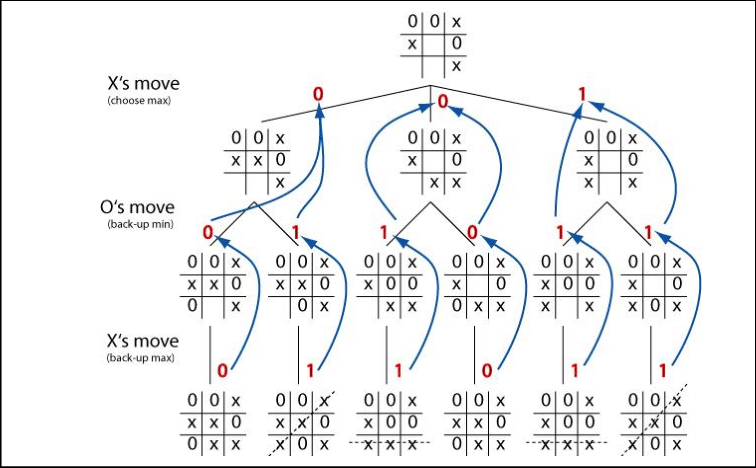
\includegraphics[width=0.89\textwidth]{images/theory/minimax_tic-tac-toe.png}
    \caption[Spielbaum eines Tic-Tac-Toe Spiels erstellt mittels des Mini-Max-Algorithmuses]{Spielbaum eines Tic-Tac-Toe Spiels erstellt mittels des Mini-Max-Algorithmuses [\cite{Elnaggar2014}]}
    \label{fig:minimax_tic-tac-toe}
\end{figure}

Die Ausgangssituation des Spiel ist an der Wurzel des Baumes abgebildet.
Im Falle des Spiels Tic-Tac-Toe wird festgelegt, dass Spieler X bestrebt ist, den Punktwert zu maximieren, wohingegen Spieler O bestrebt ist, diesen zu minimieren.
Spieler X ist als nächstes am Zug und besitzt drei Möglichkeiten, sein Kreuz auf dem Spielfeld zu platzieren.
Dem folgt der Spielzug des Spielers O, der seinerseits für jeden möglichen Spielzug von Spieler X je zwei Möglichkeiten besitzt, sein Symbol zu setzen.
Somit gibt es von der Ausgangslage her sechs mögliche Spielzüge, die Spieler O durchführen kann.
Zu guter Letzt hat Spieler X für jede seiner Ausgangslagen nur noch eine Möglichkeit, sein Kreuz zu setzen.
Jeder mögliche Endstand des Spiels erhält nun einen Punktwert.
Markiert der Endstand einen Sieg für Spieler X, so erhält dieser den Wert 1, bei einem Sieg für Spieler O den Wert -1 und bei einem Unendschieden den Wert 0.
Die Werte der Blattknoten werden anschließend nach oben propagiert.
Maximierende Knoten (Spieler X ist am Zug) übernehmen den jeweils höchsten Zahlenwert, minimierende Knoten (Spieler O ist am Zug) den niedrigsten Wert.
Am Ende dieses Prozesses ist von der Ausgangslage des Spiels erkennbar, dass Spieler X dem rechten Pfad des Baumes folgen muss, um garantiert einen Sieg zu erzielen, es für ihn aber auch bei einer Fehlentscheidung im nächsten Zug noch möglich ist, das Spiel zu gewinnen.
Beim Schach ist es jedoch in der Regel nicht möglich alle Positionen bis zum Spielende zu analysieren.
Im Gegenteil zu Tic-Tac-Toe, bei dem der Spielbaum maximal die Tiefe neun erreicht, kann beim Schach theoretisch eine Tiefe von 5899 erreicht werden [\cite{Wikipedia2018}].
Da es im Verlauf eines Schachspiels durchschnittlich $x$ mögliche Züge für den Spieler am Zug gibt, gibt es ab einer bestimmten Tiefe $t$, $x^t$ zu analysierenden Positionen.
Weil sogar schnelle Computer bei diesem exponentiell wachsenden Baum zu hohe Rechenzeiten benötigen, muss eine maximale Tiefe, bis zu der der Spielbaum analysiert wird, festgelegt werden.
Diese ist je nach Anspruch bei präzisen Evaluationen tiefer, bei schnellen Evaluationen weniger tief.
Um den Minimax Algorithmus auf Programmierebene umzusetzen, werden folgende Methoden benötigt [\cite{Shannon1950}]:

\begin{itemize}
    \item Sammelt für eine Position die erlaubten Züge. Hierfür muss sowohl auf verschiedenen Zugarten der Figuren und Schach eingegangen werden, als auch Sonderzüge wie En-Passant und die Rochade berücksichtigt werden.
    \item Die Kernaufgabe des Minimax Algorithmus umsetzt, also das abwechselnde Maximieren und Minimieren der möglichen Folgezüge einer Position.
    \item Die statische Eval-Function aus Kapitel 2.1 umsetzt.
    \item Kann für eine Position Schachzüge ausführen und diese auch rückgängig machen
\end{itemize}

Bei der Umsetzung der Kernaufgabe des Minimax-Algorithmus wird der Ansatz von [\cite{Knuth1975}] übernommen.
Außerdem wird die Standard-Implementierung verwendet, bei der der gesamte Algorithmus in zwei Prozeduren, Minimize und  Maximize, aufgeteilt wird.
Diese führen dabei jene Tätigkeiten aus, welche die Entscheidungen des minimierenden bzw. maximierenden Spielers repräsentieren.
Bei der alternativen Negamax-Implementierung gibt es nur eine Minimax-Prozedur welche die Funktionen beider Spieler übernimmt [\cite{Wikipedia2020}].
Um die Standard-Im\-ple\-men\-tie\-rung umzusetzten, werden Funktionen $F$ (Formel~\ref{eq:minimax_white-players-function-with-depth}) für den Spieler Weiß und $G$ (Formel~\ref{eq:minimax_black-players-function-with-depth}) für Spieler Schwarz definiert. Die beiden Funktionen definieren das Verhalten der Spieler beim Treffen auf eine Schachposition $p$ in der Tiefe $t$.

\begin{equation} \label{eq:minimax_white-players-function-with-depth}
    F(p,t) =
    \begin{cases}
        e(p) \quad \text{if }t=0,\\
        max(G(p1, t-1), G(p2, t-1), ... , G(pl, t-1)) \quad \text{if } t > 0
    \end{cases}
\end{equation}

\begin{equation} \label{eq:minimax_black-players-function-with-depth}
    G(p,t) =
    \begin{cases}
        e(p) \quad \text{if }t=0,\\
        min(F(p1, t-1), F(p2, t-1), ... , F(pl, t-1)) \quad \text{if } t > 0
    \end{cases}
\end{equation}

Dabei sind $p1$, ... , $pl$ die möglichen Positionen, welche nach einem Zug aus der Position p resultieren können und $e(p)$ die Bewertungsfunktion ist.
Die verwendeten Hilfsfunktionen $p.move(m)$ und $p.undoMove(m)$ führen auf der Schachstellung $p$ den Zug $m$ aus, beziehungsweise machen ihn rückgängig.
Es kann, anders als bei der Negamax-Implementierung, dieselbe Bewertungsfunktion für beide Funktionen benutzt werden, weil diese weiß-favorisierende Positionen mit positiven Werten- und schwarz-favorisierende Positionen mit negativen Werten bewertet.
Der Pseudocode für einen Minimax ist in Algorithmus~\ref{alg:minimax_minimax} dargestellt.

\begin{algorithm}[H]
    \caption{Minimax mit Tiefenbegrenzung}
    \label{alg:minimax_minimax}
    \begin{algorithmic}[1]
        \Function{maximize}{Integer $d$, Position $p$}
        \If{$d < 1$}
        \State \Return evaluate($p$)
        \Else
        \State $score \gets -\infty$
        \State $legalMoves \gets findLegalMoves(p)$
        \ForAll {$m$ in $legalMoves$}
        \State p.move(m)
        \State $moveScore \gets minimize(d-1, p)$
        \State p.undoMove(m)
        \If{$moveScore > score$}
        \State $score \gets moveScore$
        \EndIf
        \EndFor
        \EndIf
        \State \Return $score$
        \EndFunction
        \Function{minimize}{Integer $d$, Position $p$}
        \If{$d < 1$}
        \State \Return evaluate($p$)
        \Else
        \State $score \gets \infty$
        \State $legalMoves \gets findLegalMoves(p)$
        \ForAll {$m$ in $legalMoves$}
        \State p.move(m)
        \State $moveScore \gets maximize(d-1, p)$
        \State p.undoMove(m)
        \If{$moveScore < score$}
        \State $score \gets moveScore$
        \EndIf
        \EndFor
        \EndIf
        \State \Return $score$
        \EndFunction
    \end{algorithmic}
\end{algorithm}
\newpage
% !TeX root = ../../paper.tex
\subsection{Bewertungsfunktion und -heuristik}

In der Spieltheorie im Allgemeinen und im Schach im Besonderen ist es in der Regel nicht möglich, alle möglichen Zugfolgen aus einer Spielposition heraus bis zum Ende zu verfolgen.
Deshalb \glqq [...] wird eine Funktion benötigt, die die Stellung auf dem Spielbrett danach bewertet,
ob sie für eine der beiden Parteien vorteilhaft oder nachteilig ist.\grqq \ [\cite{Paulsen2009}]
Diese Funktion wird als \textit{Bewertungsfunktion} bezeichnet.
Die Bewertungsfunktion setzt sich aus einem materiellen und einer positionellen Komponente zusammen.
Bei der materiellen Komponente werden zunächst die vorhandenen weißen Figuren nach Stärke bewertet und aufsummiert.
Anschließend werden die schwarzen Figuren nach Stärke bewertet, aufsummiert und vom Gesamtwert der weißen Figuren subtrahiert.
Daraus lassen sich erste Schlussfolgerungen über den Spielstand ziehen.
Zudem ist es möglich, die derzeitige Spielphase abzuleiten [\cite{Paulsen2009}].

Da es beim Schach aber auch entscheidend ist, auf welchen Feldern sich die einzelnen Figuren befinden und in welcher Position sie zueinander stehen (Bauernstruktur, Königssicherheit), wird zusätzlich zur materiellen Komponente eine positionelle Komponente berechnet.
Die verschiedenen Positionen werden aus der Spielbrettaufstellung entnommen und fließen mit ihren jeweiligen Gewichtungen in die anschließende Bewertung ein [\cite{Paulsen2009}].


\subsubsection{Einfache Bewertungsheuristik} \label{ch:simple-eval-function}

Das Schachspiel setzt sich aus zwei wichtigen Faktoren zusammen: Einerseits ist abgesehen von der Tatsache, welcher Spieler den ersten Zug macht, keine Zufallskomponete enthalten, andererseits handelt es sich um ein Spiel mit perfekter Information.
Diese zwei Faktoren führen dazu, dass bei jeder Stellung eine der folgenden drei Aussagen gilt [\cite{Shannon1950}]:

\begin{enumerate}
    \item Es handelt sich um eine gewonnene Position für Weiß. Somit kann Weiß einen Sieg forcieren, wobei Schwarz verteidigt.
    \item Es handelt sich um eine gewonnene Position für Schwarz. Somit kann Schwarz einen Sieg forcieren, wobei Weiß spielt.
    \item Es handelt sich um eine ausgeglichene Position für beide Parteien. Somit kann es nur ein Unentschieden am Ende geben, falls beide Parteien keine Fehler machen.
\end{enumerate}

\noindent Bei einigen Spielen (so auch beim Schach) lässt sich aus den genannten zwei Faktoren und den daraus resultierenden drei Aussagen eine \textit{Bewertungsfunktion} \(\displaystyle f(P)\) ableiten, wobei \(\displaystyle P\) die Stellung bezeichnet.
Der Rückgabewert der Funktion ist die Kategorie, in die die jeweilige Position gehört: Sieg (+1), Unentschieden (0), Niederlage (-1).
Zum Zeitpunkt des Zuges des Schachcomputers werden die Werte \(\displaystyle f(P)\) für alle Positionen nach möglichen Halbzügen berechnet.
Der Zug mit dem maximalen Wert wird am Ende ausgeführt [\cite{Shannon1950}].

Es ist nicht realisierbar, alle Spielzugmöglichkeiten durchzurechnen.
Aus diesem Grund werden Approximationen der Bewertungsfunktion entworfen.
Diese Approximationen werden als Heuristiken bzw. als Bewertungsheuristiken bezeichnet.
Im Zuge dieser Arbeit wird die einfache Bewertungsheuristik nach Tomasz Michniewski verwendet, die ursprünglich in der \textit{Polish chess programming discussion list (progszach)} veröffentlicht wurde und im \href{https://www.chessprogramming.org/Main_Page}{chessprogramming.org} Wiki beschrieben wird.
Die Bewertungsheuristik ist bewusst einfach gehalten, da sie aufgrund ihrer Einfachheit schneller ist [\cite{Wiki2018}].
Die von Tomasz Michniewski beschriebene einfache Bewertungsheuristik wird in zwei Teilen dargestellt: Figurenwerte (engl. \textit{simple piece values}) und figurenspezifische Positionstabellen (engl. \textit{piece-square tables}).

Mit der Festlegung von Werten je Figur werden vier verschiedene Ziele erreicht:

\begin{enumerate}
    \item Vermeidung des Austauschs einer leichten Figur gegen drei Bauern
    \item Dem Computer signalisieren, dass das Halten des Läuferpaars vorteilhaft ist
    \item Vermeidung des Austauschs von zwei leichten Figuren gegen einen Turm und einen Bauern
    \item Ein Turm und zwei Bauern reichen aus, um gegen zwei leichte Figuren zu gewinnen
\end{enumerate}

\noindent Der erste Punkt wird durch Formel~\ref{eq:piece-values_first-result} erfüllt.

\begin{equation} \label{eq:piece-values_first-result}
\begin{split}
    L > 3B \\
    S > 3B
\end{split}
\end{equation}

\noindent Zwar gibt es durchaus Positionen, in denen drei Bauern wertvoller als eine leichte Figur sind, jedoch ist es im Allgemeinen besser eine leichte Figur zu behalten, da im Spielverlauf die Bauern individuell attackiert werden können und deren Wert als Dreier-Figuren-Gespann verloren geht [\cite{Wiki2018}].
Der zweite genannte Punkt wird durch Formel~\ref{eq:piece-values_second-result} erreicht.

\begin{equation} \label{eq:piece-values_second-result}
    L > S
\end{equation}

\noindent Zwar garantiert diese Formel kein Halten des Läuferpaars, da am Ende ein Läufer gegen einen Springer stehen kann, dennoch ist es eine Tatsache, dass Spieler oftmals Springer mit Läufern schlagen und nicht Läufer mit Springern [\cite{Wiki2018}].
Die ersten beiden Formeln~\ref{eq:piece-values_first-result} und~\ref{eq:piece-values_second-result} führen zusammen zu Formel~\ref{eq:piece-values_first-and-second-result-combined}.

\begin{equation} \label{eq:piece-values_first-and-second-result-combined}
    L > S > 3B
\end{equation}

\noindent Der dritte Punkt wird zwar durch Formel~\ref{eq:piece-values_third-result} erreicht, dennoch haben Spiele wie jenes zwischen Karpov und Kasparov gezeigt, dass bereits ein Turm und zwei Bauern ausreichen, um gegen zwei leichte Figuren gewinnen zu können.

\begin{equation} \label{eq:piece-values_third-result}
    L + S > T + B
\end{equation}

\noindent Aus diesem Grund wird die Formel~\ref{eq:piece-values_third-result}, die zu Formel~\ref{eq:piece-values_third-result-full} erweitert werden kann, um einen Faktor erweitert, woraus sich Formel~\ref{eq:piece-values_third-result-enhanced} ergibt [\cite{Wiki2018}].

\begin{equation} \label{eq:piece-values_third-result-full}
    T + 2B > L + S > T + B
\end{equation}

\begin{equation} \label{eq:piece-values_third-result-enhanced}
    L + S > T + 1.5B
\end{equation}

\noindent Durch die hier beschriebenen Formeln ist somit auch der vierte Punkt erfüllt.
Zu guter Letzt wird noch eine Formel benötigt, die das Verhältnis einer Dame-Bauer-Kombination gegenüber zwei Türmen darstellt.
Dies ist in Formel~\ref{eq:piece-values_final-result-missing} abgebildet.

\begin{equation} \label{eq:piece-values_final-result-missing}
    D + B = 2T
\end{equation}

\noindent Somit erhält man das Gleichungssystem, das in Formel~\ref{eq:piece-values_final-result} dargestellt ist.

\begin{equation} \label{eq:piece-values_final-result}
\begin{split}
    L > S > 3B \\
    L + S = T + 1.5B \\
    D + B = 2T
\end{split}
\end{equation}

\noindent Dieses Gleichungssystem wird durch die in Tabelle~\ref{tb:piece-values_satified} gelisteten Werte erfüllt.
Diese Werte wurden von Tomasz Michniewski festgelegt mit Ausnahme des Wertes des Königs.
Dieser Wert stammt aus dem Paper von Claude Shannon, wobei dieser an der Stelle dem König den Wert 200 gibt, was durch die Umrechnung in Hundertstelbauer zu 20000 führt [\cite{Shannon1950}].
Der Wert für den König ist bewusst so hoch gewählt worden, da der Verlust des Königs automatisch zur Niederlage führt.
Daraus folgt zudem, dass der Verlust des Königs durch die materielle Komponente der Bewertungsheuristik einfacher erkannt werden kann.
Zu guter Letzt sei angemerkt, dass die Wahl der Figurenwerte dazu führt, dass diese in einer 2~Byte vorzeichenbehafteten Ganzzahl abgelegt werden können, da der Gesamtwert aller Spielfiguren einer Seite rund 30300 beträgt [\cite{Wiki2018}].

\begin{table}
    \centering
    \begin{tabular}{| L{0.47\textwidth} | R{0.47\textwidth} |}
        \hline
        \thead{Figur} & \thead{Wert} \\
        \hline
        Bauer & 100 \\
        \hline
        Springer & 320 \\
        \hline
        Läufer & 330 \\
        \hline
        Turm & 500 \\
        \hline
        Dame & 900 \\
        \hline
        König & 20000 \\
        \hline
    \end{tabular}
    \caption[Figurenwerte in Hundertstelbauer]{Figurenwerte in Hundertstelbauer [\cite{Wiki2018}]}
    \label{tb:piece-values_satified}
\end{table}

Nachdem die Figurenwerte ausführlich dargelegt wurden, werden nun figurenspezifische Positionstabellen erstellt.
Diese haben die Aufgabe für gut positionierte Figuren eine \textit{Belohnung} und für schlecht positionierte Figuren \textit{Abzüge} zu erteilen [\cite{Wiki2018}].

Für die Bauern gilt, dass deren Vorwärtsbewegung prinzipiell belohnt wird.
Des Weiteren werden die zentralen Bauern (D2, E2) negativ bewertet, sollten sie sich nicht bewegen.
Das rührt daher, da Bauern direkt vor dem König-Dame-Paar als hindernd angesehen werden, weil es im Besonderen den Bewegungsfreiraum der beiden Läufer zu Beginn des Spiels einschränkt.[\cite{Wiki2018}].
Formel~\ref{eq:piece-squared-tables_pawns-matrix} zeigt mittels einer Matrix die positionsbezogenen Werte für Bauern auf dem Spielbrett.

\begin{equation} \label{eq:piece-squared-tables_pawns-matrix}
\begin{pmatrix}
0 & 0 & 0 & 0 & 0 & 0 & 0 & 0 \\
50 & 50 & 50 & 50 & 50 & 50 & 50 & 50 \\
10 & 10 & 20 & 30 & 30 & 20 & 10 & 10 \\
5 & 5 & 10 & 25 & 25 & 10 & 5 & 5 \\
0 & 0 & 0 & 20 & 20 & 0 & 0 & 0 \\
5 & -5 & -10 & 0 & 0 & -10 & -5 & 5 \\
5 & 10 & 10 & -20 & -20 & 10 & 10 & 5 \\
0 & 0 & 0 & 0 & 0 & 0 & 0 & 0
\end{pmatrix}
\end{equation}

\bigskip

\noindent Eine genauere Erläuterung zu den einzelnen Werten pro Spielposition der Bauern kann bei [\cite{Wiki2018}] nachgelesen werden.

Springer sind aufgrund ihrer Bewegungsart am effektivsten in der Mitte des Spielfeldes, weshalb sie auf den mittleren Positionen höhere Punktwerte erhalten.
Demgegenüber erhalten sie negative Punktwerte für Randpositionen, da diese ihren Bewegungsradius einschränken [\cite{Wiki2018}].
Formel~\ref{eq:piece-squared-tables_knights-matrix} zeigt die entsprechenden Werte für die Springerpositionen.

\begin{equation} \label{eq:piece-squared-tables_knights-matrix}
\begin{pmatrix}
-50 & -40 & -30 & -30 & -30 & -30 & -40 & -50 \\
-40 & -20 & 0 & 0 & 0 & 0 & -20 & -40 \\
-30 & 0 & 10 & 15 & 15 & 10 & 0 & -30 \\
-30 & 5 & 15 & 20 & 20 & 15 & 5 & -30 \\
-30 & 0 & 15 & 20 & 20 & 15 & 0 & -30 \\
-30 & 5 & 10 & 15 & 15 & 10 & 5 & -30 \\
-40 & -20 & 0 & 5 & 5 & 0 & -20 & -40 \\
-50 & -40 & -30 & -30 & -30 & -30 & -40 & -50
\end{pmatrix}
\end{equation}

\bigskip

\noindent Läufer erhalten zusätzliche Punkte für zentrale Positionen, da sie dort, ähnlich wie Springer, den größten Bewegungsradius besitzen.
Des Weiteren erhalten sie für Randpositionen Abzüge, wobei die Positionen in den Ecken des Spielbretts besonders negativ bewertet sind [\cite{Wiki2018}].
Eine positionsbezogene Punktwerteaufstellung mittels einer Matrix ist in Formel~\ref{eq:piece-squared-tables_bishops-matrix} abgebildet.

\begin{equation} \label{eq:piece-squared-tables_bishops-matrix}
\begin{pmatrix}
-20 & -10 & -10 & -10 & -10 & -10 & -10 & -20 \\
-10 & 0 & 0 & 0 & 0 & 0 & 0 & -10 \\
-10 & 0 & 5 & 10 & 10 & 5 & 0 & -10 \\
-10 & 5 & 5 & 10 & 10 & 5 & 5 & -10 \\
-10 & 0 & 10 & 10 & 10 & 10 & 0 & -10 \\
-10 & 10 & 10 & 10 & 10 & 10 & 10 & -10 \\
-10 & 5 & 0 & 0 & 0 & 0 & 5 & -10 \\
-20 & -10 & -10 & -10 & -10 & -10 & -10 & -20
\end{pmatrix}
\end{equation}

\bigskip

\noindent Tomasz Michniewski weißt den Türmen keine stark unterschiedlichen positionsbezogenen Punktwerte zu, wie er dies bei den Springern und Läufern tut.
Die Türme erhalten lediglich einen Bonus für den siebten Rang und negative Werte für die Außenpositionen A und H [\cite{Wiki2018}] (siehe Formel~\ref{eq:piece-squared-tables_rooks-matrix}).

\begin{equation} \label{eq:piece-squared-tables_rooks-matrix}
\begin{pmatrix}
0 & 0 & 0 & 0 & 0 & 0 & 0 & 0 \\
5 & 10 & 10 & 10 & 10 & 10 & 10 & 5 \\
-5 & 0 & 0 & 0 & 0 & 0 & 0 & -5 \\
-5 & 0 & 0 & 0 & 0 & 0 & 0 & -5 \\
-5 & 0 & 0 & 0 & 0 & 0 & 0 & -5 \\
-5 & 0 & 0 & 0 & 0 & 0 & 0 & -5 \\
-5 & 0 & 0 & 0 & 0 & 0 & 0 & -5 \\
0 & 0 & 0 & 5 & 5 & 0 & 0 & 0
\end{pmatrix}
\end{equation}

\bigskip

\noindent Die Erstellung einer Figuren-Quadrat Tabelle für die Dame dient nicht dazu, gute Stellungen zu belohnen, sondern schlechte mit Abzügen zu versehen.
Dennoch lässt sich aus der von Tomasz Michniewski aufgestellten Darstellung ableiten, dass die Dame in der Mitte des Spielbretts aufhalten sollte [\cite{Wiki2018}] (siehe Formel~\ref{eq:piece-squared-tables_queen-matrix}).

\begin{equation} \label{eq:piece-squared-tables_queen-matrix}
\begin{pmatrix}
-20 & -10 & -10 & -5 & -5 & -10 & -10 & -20 \\
-10 & 0 & 0 & 0 & 0 & 0 & 0 & -10 \\
-10 & 0 & 5 & 5 & 5 & 5 & 0 & -10 \\
-5 & 0 & 5 & 5 & 5 & 5 & 0 & -5 \\
0 & 0 & 5 & 5 & 5 & 5 & 0 & -5 \\
-10 & 5 & 5 & 5 & 5 & 5 & 0 & -10 \\
-10 & 0 & 5 & 0 & 0 & 0 & 0 & -10 \\
-20 & -10 & -10 & -5 & -5 & -10 & -10 & -20
\end{pmatrix}
\end{equation}

\bigskip

\noindent Zu guter Letzt werden zwei figurenspezifische Positionstabellen für den König aufgestellt.
Die erste Tabelle (siehe Formel~\ref{eq:piece-squared-tables_king-matrix-1}) ist für mittlere Phase des Spiels gedacht.
Hierbei wird deutlich, dass der König zurückgehalten und hinter der Bauernlinie gehalten werden sollte [\cite{Wiki2018}].

\begin{equation} \label{eq:piece-squared-tables_king-matrix-1}
\begin{pmatrix}
-30 & -40 & -40 & -50 & -50 & -40 & -40 & -30 \\
-30 & -40 & -40 & -50 & -50 & -40 & -40 & -30 \\
-30 & -40 & -40 & -50 & -50 & -40 & -40 & -30 \\
-30 & -40 & -40 & -50 & -50 & -40 & -40 & -30 \\
-20 & -30 & -30 & -40 & -40 & -30 & -30 & -20 \\
-10 & -20 & -20 & -20 & -20 & -20 & -20 & -10 \\
20 & 20 & 0 & 0 & 0 & 0 & 20 & 20 \\
20 & 30 & 10 & 0 & 0 & 10 & 30 & 20
\end{pmatrix}
\end{equation}

\bigskip

\noindent Für die Endspielphase sieht die Tabelle für den König jedoch anders aus (siehe Formel~\ref{eq:piece-squared-tables_king-matrix-2}).
Randpositionen schränken den König in seiner Bewegung zusätzlich ein und sind gerade in der Endphase von erhöhtem Risiko, weshalb diese Positionen besonders negativ bewertet sind.
Demgegenüber sind die zentralen Positionen besonders positiv bewertet [\cite{Wiki2018}].

\begin{equation} \label{eq:piece-squared-tables_king-matrix-2}
\begin{pmatrix}
-50 & -40 & -30 & -20 & -20 & -30 & -40 & -50 \\
-30 & -20 & -10 & 0 & 0 & -10 & -20 & -30 \\
-30 & -10 & 20 & 30 & 30 & 20 & -10 & -30 \\
-30 & -10 & 30 & 40 & 40 & 30 & -10 & -30 \\
-30 & -10 & 30 & 40 & 40 & 30 & -10 & -30 \\
-30 & -10 & 20 & 30 & 30 & 20 & -10 & -30 \\
-30 & -30 & 0 & 0 & 0 & 0 & -30 & -30 \\
-50 & -30 & -30 & -30 & -30 & -30 & -30 & -50
\end{pmatrix}
\end{equation}

\bigskip

\noindent Zusätzlich zu den eben beschriebenen figurenspezifischen Positionstabellen beschreibt Tomasz Michniewski, wann die Endphase des Spiel beginnt.
Diese beginnt nach ihm, wenn eine der beiden folgenden Aussagen zutrifft [\cite{Wiki2018}]:

\begin{enumerate}
    \item Beide Seiten besitzen keine Dame
    \item Beide Seiten haben neben der Dame entweder keine weiteren Figuren oder aber maximal eine leichte Figur
\end{enumerate}

% !TeX root = ../../paper.tex
\subsection{Mini-Max-Suche}

Im Schachspiel ist jeder Spieler bestrebt, das für ihn bestmögliche Spielergebnis zu erzielen.
Zur Abbildung dieses Prinzips dient der \textit{Mini-Max}-Algorithmus [\cite{Paulsen2009}].
Um dies abbilden zu können wird ein Punktwert eingeführt, den ein Spieler zu maximieren versucht und der andere Spiele zu minimieren versucht.
Für das Schachspiel und die spätere Betrachtung dessen wird an dieser Stelle festgelegt, dass eine hohe Bewertungen für einen Vorteil der weißen Spielseite steht, wohingegen eine negative Bewertungen für einen Vorteil für die schwarze Spielseite steht.
Somit ist Weiß bestrebt, den Wert durch die Wahl einer Spieloption zu maximieren und Schwarz den Wert zu minimieren [\cite{Paulsen2009}].
Zur Berechnung dieses Punktwertes wird ein Spielbaum (engl. \textit{game tree}) benötigt, der alle möglichen Spielzüge beinhaltet.
Es werden alle Knoten eines Spielbaumes mit ihren zugehörigen Werten generiert [\cite{Shah2007}].
Die Knoten innerhalb des Baumes werden in drei verschiedene Kategorien unterteilt: Blattknoten, minierende und maximierende Knoten.
Jeder Blattknoten erhält seinen Nutzwert (engl. \textit{utility value}).
Den minimierenden Knoten wird jeweils der kleinste Wert ihrer Kindknoten zugewiesen, den maximierenden Knoten jeweils der größte Wert [\cite{Shah2007}].
Abbildung~\ref{fig:minimax_tic-tac-toe} zeigt einen Teil eines Spielbaums für das Spiel Tic-Tac-Toe, der die einzelnen Schritte der Berechnung durch den Mini-Max-Algorithmus beinhaltet.

\begin{figure}
    \centering
    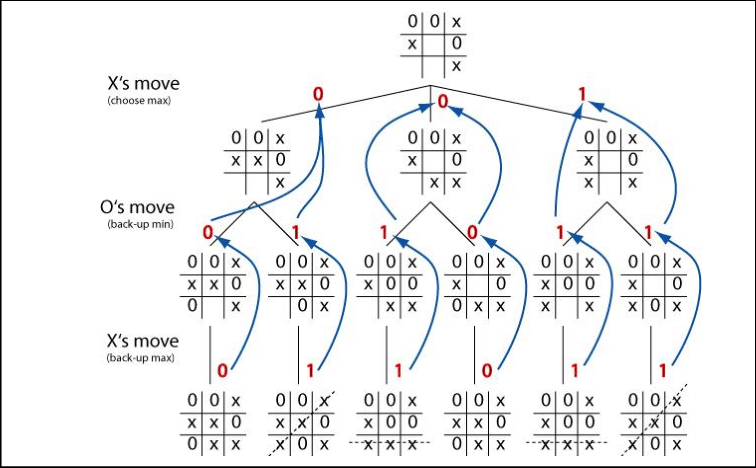
\includegraphics[width=0.89\textwidth]{images/theory/minimax_tic-tac-toe.png}
    \caption[Spielbaum eines Tic-Tac-Toe Spiels erstellt mittels des Mini-Max-Algorithmuses]{Spielbaum eines Tic-Tac-Toe Spiels erstellt mittels des Mini-Max-Algorithmuses [\cite{Elnaggar2014}]}
    \label{fig:minimax_tic-tac-toe}
\end{figure}

Die Ausgangssituation des Spiel ist an der Wurzel des Baumes abgebildet.
Im Falle des Spiels Tic-Tac-Toe wird festgelegt, dass Spieler X bestrebt ist, den Punktwert zu maximieren, wohingegen Spieler O bestrebt ist, diesen zu minimieren.
Spieler X ist als nächstes am Zug und besitzt drei Möglichkeiten, sein Kreuz auf dem Spielfeld zu platzieren.
Dem folgt der Spielzug des Spielers O, der seinerseits für jeden möglichen Spielzug von Spieler X je zwei Möglichkeiten besitzt, sein Symbol zu setzen.
Somit gibt es von der Ausgangslage her sechs mögliche Spielzüge, die Spieler O durchführen kann.
Zu guter Letzt hat Spieler X für jede seiner Ausgangslagen nur noch eine Möglichkeit, sein Kreuz zu setzen.
Jeder mögliche Endstand des Spiels erhält nun einen Punktwert.
Markiert der Endstand einen Sieg für Spieler X, so erhält dieser den Wert 1, bei einem Sieg für Spieler O den Wert -1 und bei einem Unendschieden den Wert 0.
Die Werte der Blattknoten werden anschließend nach oben propagiert.
Maximierende Knoten (Spieler X ist am Zug) übernehmen den jeweils höchsten Zahlenwert, minimierende Knoten (Spieler O ist am Zug) den niedrigsten Wert.
Am Ende dieses Prozesses ist von der Ausgangslage des Spiels erkennbar, dass Spieler X dem rechten Pfad des Baumes folgen muss, um garantiert einen Sieg zu erzielen, es für ihn aber auch bei einer Fehlentscheidung im nächsten Zug noch möglich ist, das Spiel zu gewinnen.
Beim Schach ist es jedoch in der Regel nicht möglich alle Positionen bis zum Spielende zu analysieren. Im Gegenteil zu Tic-Tac-Toe, bei dem der Spielbaum maximal die Tiefe neun erreicht, kann beim Schach theoretisch eine Tiefe von 5899 erreicht werden (Quelle Wikipedia 50-Züge-Regel).
Da es im Verlauf eines Schachspiels durchschnittlich $x$ mögliche Züge für den Spieler am Zug gibt, gibt es ab einer bestimmten Tiefe $t$, $x^t$ zu analysierenden Positionen !Quelle Shannon number. Weil sogar schnelle Computer bei diesem exponentiell wachsenden Baum irgendwann zu hohe Rechenzeiten benötigen, muss man sich auf eine maximale Tiefe festlegen bis zu der man den Spielbaum analysiert. Diese ist je nach Anspruch, bei präzisen Evaluationen tiefer, bei schnellen Evaluationen weniger tief.\\.
Um den Minimax Algorithmus auf Programmierebene umzusetzen, werden folgende Methoden benötigt (Quelle Shannon).
\begin{itemize}
    \item Sammelt für eine Position die erlaubten Züge. Hierfür muss sowohl auf verschiedenen Zugarten der Figuren und Schach eingegangen werden, als auch Sonderzüge wie En-Passant und die Rochade berücksichtigt werden.
    \item Die Kernaufgabe des Minimax Algorithmus umsetzt, also das abwechselnde Maximieren und Minimieren der möglichen Folgezüge einer Position.
    \item Die statische Eval-Function aus Kapitel 2.1 umsetzt.
\end{itemize}
Beim Umsetzen der Kernaufgabe des Minimax-Algorithmus wird der Ansatz von Knuth und Moore übernommen.
Es werden Funktionen $F$ und $G$ für für beide Spieler (Weiß und Schwarz)  definiert, welche ihr Verhalten beim Treffen auf eine Schachposition $p$ in der Tiefe $t$ definiert.
\begin{equation*}
    F(p,t) =
    \begin{cases}
        e(p) \quad \text{if }t=0,\\
        max(G(p1, t-1), G(p2, t-1), ... , G(pl, t-1)) \quad \text{if } t > 0
    \end{cases}
\end{equation*}
\begin{equation*}
    G(p,t) =
    \begin{cases}
        e(p) \quad \text{if }t=0,\\
        min(F(p1, t-1), F(p2, t-1), ... , F(pl, t-1)) \quad \text{if } t > 0
    \end{cases}
\end{equation*}
wobei $p1$, ... , $pl$ die möglichen Positionen sind, welche nach einem Zug aus der Position p resultieren können und $e(p)$ die Eval-Function ist. Es kann dieselbe Eval-Function für beide Funktionen benutzt werden, weil diese weiß-favorisierende Positionen mit positiven Werten- und schwarz-favorisierende Positionen mit negativen Werten bewertet.
In Pseudocode sieht ein Minimax folgendermaßen aus:

\begin{algorithm}
    \caption{Minimax}
    \begin{algorithmic}[1]
        \Function{maximize}{Integer $d$, Position $p$}
        \If{$d < 1$}
        \State \Return evaluate($p$)
        \Else
        \State $score \gets -\infty$
        \State $legalMoves \gets findLegalMoves(p)$
        \ForAll {$m$ in $legalMoves$}
        \State p.move(m)
        \State $moveScore \gets minimize(d-1, p)$
        \If{$moveScore > score$}
        \State $score \gets moveScore$
        \EndIf
        \EndFor
        \EndIf
        \State \Return $score$
        \EndFunction
        \Function{minimize}{Integer $d$, Position $p$}
        \If{$d < 1$}
        \State \Return evaluate($p$)
        \Else
        \State $score \gets \infty$
        \State $legalMoves \gets findLegalMoves(p)$
        \ForAll {$m$ in $legalMoves$}
        \State p.move(m)
        \State $moveScore \gets maximize(d-1, p)$
        \If{$moveScore < score$}
        \State $score \gets moveScore$
        \EndIf
        \EndFor
        \EndIf
        \State \Return $score$
        \EndFunction
    \end{algorithmic}
\end{algorithm}

% !TeX root = ../../paper.tex
\subsubsection{Vorsortieren}

Damit der Alpha-Beta Algorithmus, der in Kapitel~\ref{ch:alpha-beta-pruning} beschrieben wurde, bestmöglich wirken kann, müssen die aussichtsreichsten Züge zuerst durchsucht werden [\cite{Wiki2019}].
Es existieren verschiedenste Herangehensweisen, dies umzusetzen.
Da die möglichen Spielzüge in einem Suchgraphen abgebildet werden können und ein Schachcomputer für den allgemeinen Bedarf möglichst wenig Speicher benötigen sollte, bietet sich das \textit{Depth-First} Suchverfahren (zu dt. etwa \textit{Tiefensuche}) an.
Dabei werden zuerst tieferliegende Knoten ausgewertet, bevor benachbarte Knoten ausgewertet werden.
Das Depth-First Verfahren bietet den Vorteil, dass nur jeweils ein Pfad des Baumes im Speicher gehalten werden muss [\cite{Wiki2019b}].
Abbildung~\ref{fig:pre-sorting_depth-first-tree} zeigt eine beispielhafte Evaluierung eines Baumes nach dem Depth-First Verfahren.

\begin{figure}[H]
    \centering
    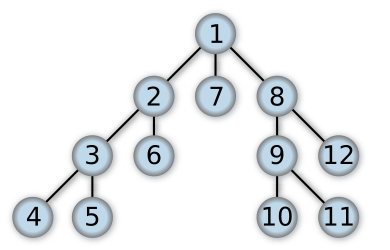
\includegraphics[width=0.6\textwidth]{images/theory/pre-sorting_depth-first-tree.png}
    \caption[Beispielhafter Depth-First Baum]{Beispielhafter Depth-First Baum [\cite{Wiki2019b}]}
    \label{fig:pre-sorting_depth-first-tree}
\end{figure}

\noindent Die Zahlen innerhalb der Knoten repräsentieren die Reihenfolge, in der die Knoten besucht werden.
Im Beispiel wird zuerst der Wurzelknoten betrachtet.
Von diesem ausgehend wir der am weitesten links befindliche Kindknoten evaluiert (markiert durch die Zahl 2).
Der nächstfolgende Knoten ist wiederum der am weitesten links befindliche Kindknoten, in der Abbildung markiert durch die Zahl 3.
Nachdem der Knoten mit der Zahl 4 evaluiert wurde, ist die maximale Tiefe für diesen Pfad erreicht, da der Knoten mit der Zahl 4 keine Kindknoten besitzt.
Aus diesem Grund wird eine Ebene höher beim Knoten mit der Zahl 3 geschaut, ob dieser noch weitere Kindknoten besitzt.
Da dies der Fall ist, werden jene weiteren Kindknoten evaluiert.
Im abgebildeten Beispiel betrifft dies ausschließlich den Knoten mit der Zahl 5.
Da weder Knoten 5 noch eine Ebene höher Knoten 3 weitere Kindknoten besitzen, wird wieder eine Ebene weiter oben geschaut.
Dieser Prozess wird solange fortgeführt, bis alle Knoten besucht wurden.

Weil ein Schachcomputer, der in einem Spiel gegen einen Menschen Einsatz findet, in einer für seinen Gegner vertretbaren Zeit antworten muss, werden Zeitmanagementstrategien benötigt.
Diese legen fest, in welcher Reihenfolge die möglichen Spielzüge ausgewerten werden, um die aussichtsreichsten Spielzüge möglichst am Anfang durchzurechnen.
Bei den Depth-First Suchverfahren hat sich das \textit{Iterative Deepening} (zu dt. etwa \textit{iterative Tiefensuche}) als grundlegende Zeitmanagementstrategie durchgesetzt.
Bei dieser Zeitmanagementstrategie werden alle möglichen Pfade eines Spielbaumes bis zu einer Tiefe von~1 ausgewertet.
Ist nach Abschluss der Auswertung die verfügbare Zeit des Spielzugs noch nicht abgelaufen, so wird die Suchtiefe um eins erhöht und eine weitere Evaluierungsphase beginnt [\cite{Wiki2019a}].
Abbildung~\ref{fig:pre-sorting_iterative-deepening} stellt diesen Vorgang grafisch an einem Beispiel dar.

\begin{figure}[H]
    \centering
    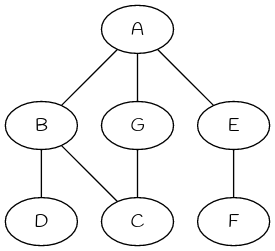
\includegraphics[width=0.6\textwidth]{images/theory/pre-sorting_iterative-deepening.png}
    \caption[Grafische Darstellung der Zeitmanagementstrategie Iterative Deepening]{Grafische Darstellung der Zeitmanagementstrategie Iterative Deepening}
    \label{fig:pre-sorting_iterative-deepening}
\end{figure}

\noindent Bei der folgenden beispielhafter Erläuterung des Iterative Deepening wird angenommen, dass die Knoten von links nach recht abgearbeitet werden.
Im ersten Durchlauf werden bei einer Tiefe von~1 nur die Knoten A B G und E evaluiert.
Somit sind dem Schachcomputer jetzt bereits alle möglichen Spielzüge bis zu einer Tiefe von eins bekannt, sodass er bei Abbruch des Spielzuges aufgrund der abgelaufenen Zeit bereits eine mögliche gute Entscheidung fällen kann.
Darstellung~\ref{eq:pre-sorting_iterative-deepening-example} zeigt die Reihenfolge der ausgewerteten Knoten für die Tiefen~2 und~3.

\begin{align} \label{eq:pre-sorting_iterative-deepening-example}
\begin{split}
    & \text{Tiefe 2: } A\ B\ D\ C\ G\ C\ E\ F\\
    & \text{Tiefe 3: } A\ B\ D\ C\ G\ G\ C\ B\ E\ F
\end{split}
\end{align}

\subsubsection{Ruhesuche}

Eine weitere Methode den Minimax Algorithmus zu verbessern ist die sogenannte Ruhesuche.
Im Schach kommt es oftmals zu erzwungenen Zugsequenzen (engl. \textit{forced line}).
Das bedeutet, dass die ziehende Seite eine eingeschränkte Wahl hat zu ziehen.
Diese Situation tritt beispielsweise auf, wenn der eigene König im Schach steht oder weil dem Gegner sonst eine vorteilhafte Position ermöglicht wird.
Ein Problem entsteht nun, wenn die Analysetiefe des Spielbaums mitten in einer erzwungenen Zugsequenzen endet, denn dann liefert die Analyse keine aussagekräftige Evaluation.

Es werden deshalb drei Fälle definiert, bei dessen Eintreffen die Standardsuchtiefe erweitert wird [\cite{Stuckardt}]:

\begin{enumerate}
    \item Der ziehende Spieler befindet sich im Schach.
    \item Der ziehende Spieler kann mit einem Bauern die letzte Reihe erreichen und diesen befördern.
    \item Der ziehende Spieler kann einen potenziell vorteilhaften Schlagzug tätigen.
\end{enumerate}

Die ersten beiden Kriterien sind selbsterklärend, mit der Ausnahme, dass beim befördern der Bauern nur der Fall Dame und der Fall Springer berücksichtigt werden.
Grund hierfür ist, dass die Bewegungsmöglichkeiten des Turms und des Läufers beide in denen der Dame enthalten sind.
Es gibt zwar Situationen, in denen durch Pattgefahr ein Unterbefördern (engl. \textit{underpromote}) in einen Turm beziehungsweise Läufer sinnvoll ist, allerdings ist das eine Seltenheit und es lohnt sich nicht dafür den Spielbaum aufzublähen [\cite{Stuckardt}].
Das dritte Kriterium wird im Folgenden erläutert.

Erfahrene Schachspieler opfern selten Figuren, ohne dafür etwas im Gegenzug zu erhalten.
Aus diesem Grund sind die meisten Schlagzüge im Schach sogenannte Figurenabtausche.
Hier schlägt beispielsweise Weiß eine Figur von Schwarz, welche dann wiederum eine Figur von Weiß, meistens mit ähnlichem Wert, schlägt, sodass nach dem Abtausch wieder ein ähnliches Kräftegleichgewicht herrscht wie vor dem Abtausch.
Oftmals folgen mehrere Abtausche aufeinander, bei dem dann mehr als nur zwei Figuren geschlagen werden.
Ein vorteilhafter Schlagzug ist nun ein Schlagzug, bei dem entweder

\begin{enumerate}
    \item die geschlagene Figur wertvoller ist als die Figur, welche schlägt, oder
    \item die angegriffene Figur von weniger gegnerischen Figuren verteidigt wird, als sie von eigenen Figuren bedroht wird. Dies kann dazu führen, dass der initiale Schlagzug nicht unbedingt einen direkten Vorteil bringt, der gesamte Figurenabtausch jedoch schon [\cite{Shannon1950}][\cite{Stuckardt}].
\end{enumerate}

\def\Quiescence{ra8, bc8, qd8, rf8, kg8, pa6, pb7, pc7, pd6, pf7, pg7, ph7, nf6, nd5, Pa4, Nb3, Pb2, Pc2, Rd1, Be2, Pe3, Qf3, Pf2, Pg2, Ph2, Ng3, Rf1, Kg1}
\setchessboard{setpieces=\Quiescence}
\begin{center}
    \chessboard[largeboard, pgfstyle=straightmove, color=red ,linewidth=0.1em,markmove={d1-d5,f3-d5}, color=green,pgfstyle=knightmove, markmove= f6-d5]
\end{center}

Kriterium a) ist sehr intuitiv verständlich, da der Tausch einer weniger wertvollen Figur für eine wertvollere per Definition vorteilhaft ist, sofern keine anderen negativen Konsequenzen daraus folgen.

Kriterium b) ist da schon etwas komplizierter.
Hier werden auch Schlagzüge betrachtet, welche gleichwertige oder, wie im oberen Beispiel dargestellt, sogar weniger wertvolle Figuren schlagen, solange das Schlagfeld feldbeherrschungstechnisch majorisiert wird [\cite{Stuckardt}].

Im Beispiel sieht dann der Figurenabtausch folgendermaßen aus: Weiß schlägt den gegnerischen Springer auf d5 mit dem Turm auf d1. Anschließend schlägt Schwarz mit dem Springer auf f6 zurück und zuletzt schlägt Weiß diesen Springer mit der Dame auf f3.
Am Schluss dieses Abtausches hat Schwarz zwei Springer (6 Bauern) verloren und Weiß einen Turm (5 Bauern).
Der Tausch favorisiert also Weiß, obwohl der initiale Schlagzug zunächst nicht vorteilhaft ist.

Hierbei ist außerdem wichtig zu erwähnen, dass ein Figurentausch nach Kriterium 2. nicht notwendigerweise zu einem favorisierenden Ergebnis für den Spieler mit der Feldbeherrschung führt.
Nehmen wir nämlich an, im oben beschriebenen Beispiel steht auf d5 zu Beginn kein schwarzer Springer, sondern ein schwarzer Bauer, so würde der gleiche Abtausch mit einem Verlust von 4 Bauern für Schwarz (Bauer + Springer) und einem Verlust von 5 Bauern für weiß (Turm) resultieren, obwohl sich die Feldbeherrschung nicht geändert hat.
Des Weiteren muss die Stellungsdarstellung bereits jene Schlagmöglichkeiten vorher erkennen, die sich im Verlauf des Figurenabtausches offenbaren können.
Dies tritt beispielsweise auf, wenn sie vorher durch eigene Figuren blockiert wurden (sogennante \textit{Batterien}) [\cite{Stuckardt}].

Die Ruhesuche wird nun so implementiert, dass bis zu einer maximalen Tiefe von 30 Halbzügen nach einer Ruhestellung, die keine der drei Bedingungen zulässt, gesucht wird.
Bei dieser Tiefe wurde empirisch gezeigt, dass die meisten Positionen bereits zu einer Ruhestellung gekommen sind.
Die Selektivität von Kriterium a) und b) ist stark genug, sodass gegebenenfalls auftretende Effizienzprobleme vernachlässigbar sind [\cite{Stuckardt}].

% !TeX root = ../../paper.tex
\subsubsection{Transpositionstabellen} \label{ch:transposition-tables}

Im Schach treten viele \textit{Transpositionen} auf.
Transpositionen sind verschiedene Permutationen einer Zugsequenz, die in die selbe Stellung münden [\cite{Russell2010}].
Folgendes Beispiel soll dies näher illustrieren: Weiß hat einen Zug, $a1$, der von Schwarz mit $b1$ beantwortet werden kann, und einen nicht verwandten Zug $a2$ auf der anderen Seite des Bretts, der mit $b2$ beantwortet werden kann.
Beide Sequenzen $[a1, b1, a2, b2]$ und $[a2, b2, a1, b1]$ münden in der gleichen Stellung.
Es ist vorteilhaft, das Ergebnis der ersten Zugsequenz in einer Hashtabelle abzulegen und beim zweiten Mal das Ergebnis aus der Hash Tabelle zu verwenden, anstatt es von Neuem zu berechnen.
Das Verwenden von Transpositionstabellen kann einen signifikanten Einfluss haben.
So kann die Verwendung dafür sorgen, dass in einigen Fällen der Schachcomputer bis zu der doppelten Tiefe suchen kann [\cite{Russell2010}].

In der Hashtabelle wird ein eindeutiger Schlüssel zur Identifikation eines Eintrags verwendet.
Im Falle der Transpositionstabellen wird dabei die Stellung als Schlüssel verwendet.
Die Stellung muss hierbei mittels einer Hashfunktion in einen Schlüssel umgewandelt werden.
Hierfür exisitieren verschiedenste Ansätze und Hashfunktionen.
Zu den bekanntesten zählen Zobrist Hashing und BCH Hashing [\cite{Wiki2020}].
Im Zuge dieser Arbeit Zobrist Hashing verwendet.
Als eindeutiger Schlüssel wird ein Tupel bestehend aus dem Hash und der Tiefe verwendet.

Als Wert zum Schlüssel wird ein Tripel der Form $<score, alpha, beta>$ gespeichert.
Es ist von entscheidender Bedeutung, dass nicht nur der Score abgespeichert wird, sondern auch die dazugehörigen Intervallsgrenzen Alpha und Beta, um überprüfen zu können, ob der Score an der verwendeten Stelle aussagekräftig genug ist [\cite{Wiki2020}].
Liegen das für eine Stellung verwendete Alpha-Beta-Intervall innerhalb eines abgespeicherten Intervalls für diese Stellung oder ist mit dem gespeicherten Intervall identisch, so darf der abgelegte Wert verwendet werden.
Andernfalls wird das Intervall angepasst und der Score muss von Neuem berechnet werden.

Da die Menge an Transpositionstabellen zu groß für einen Heimcomputer werden kann, muss eine maximale Anzahl von Transpositionstabellen im Speicher festgelegt werden.
Zudem muss ein Verfahren bestimmt und implementiert werden, wann Transpositionstabellen aus dem Speicher entfernt werden.
Hierfür eignet sich der \ac{LRU} Ansatz.
Das bedeutet, dass, falls die maximale Anzahl an Einträgen erreicht ist, der Eintrag, der am längsten nicht verwendet wird, aus dem Speicher entfernt wird und Platz für den neuen Eintrag schafft.
Eine Implementierung dieses Verfahrens in Python ist in Listing~\ref{lst:transpo-tables_lru-cache} dargestellt.

\bigskip

\begin{lstlisting}[caption={Implementierung eines LRU Caches}, captionpos=b, label={lst:transpo-tables_lru-cache}, language=Python]
class LRUCache:
    def __init__(self, size):
        self.od = OrderedDict()
        self.size = size

    def get(self, key, default=None):
        try:
            self.od.move_to_end(key)
        except KeyError:
            return default
        return self.od[key]
    
    def __contains__(self, item):
        return item in self.od
    
    def __len__(self):
        return len(self.od)

    def __getitem__(self, key):
        self.od.move_to_end(key)
        return self.od[key]

    def __setitem__(self, key, value):
        try:
            del self.od[key]
        except KeyError:
            if len(self.od) == self.size:
                self.od.popitem(last=False)
        self.od[key] = value
\end{lstlisting}

\noindent Es handelt sich um einen klassenbasierten Ansatz, wobei intern zur Speicherung ein \lstinline[language=Python]{OrderedDict} verwendet.
Der Vorteile eine \lstinline[language=Python]{OrderedDict} gegenüber eines normalen Dictionary ist die Tatsache, dass ein \lstinline[language=Python]{OrderedDict} sich die Reihenfolge, in der neue Schlüssel-Wert-Paare hinzugefügt werden, merkt.
An dieser Stelle wird ein Wrapper für das \lstinline[language=Python]{OrderedDict} verwendet, um den Alterungsprozess von Einträgen kontrollieren zu können.
Wird auf einen bereits vorhandenen Eintrag zugegriffen, so wird dieser erst an das Ende des \lstinline[language=Python]{OrderedDict} verschoben und dann zurückgegeben.
Wird hingegen ein neuer Eintrag hinzugefügt, obwohl die maximale Anzahl an Einträgen bereits erreicht ist, so wird das erste Element im \lstinline[language=Python]{OrderedDict}, das somit am längsten nicht verwendet wurde, gelöscht und der neue Eintrag am Ende eingefügt.

Die in Listing~\ref{lst:transpo-tables_lru-cache} dargestellte Implementierung eines \ac{LRU} Caches wird in der späteren Umsetzung der Transpositionstabellen verwendet.

